\documentclass[conference]{IEEEtran}
\usepackage{polyglossia}
\usepackage{moreverb}
\usepackage{mathtools}
\usepackage{amsfonts}
\usepackage{pifont}
\usepackage{booktabs,caption}
\captionsetup{labelsep=newline,singlelinecheck=false} % optional
\usepackage{tabularx}

\begin{document}
\title{A Discussion of the Robust Information-theoretic Clustering Framework (RIC)}
\author{\IEEEauthorblockN{Simon Lackerbauer}
\IEEEauthorblockA{Institut für Informatik\\
Ludwig-Maximilians-Universität München\\
Oettingenstraße 67, 80538 München\\
lackerbauer@lrz.mwn.de}}

\maketitle

\begin{abstract}
In the 2006 paper \textit{Robust Information-theoretic Clustering} Böhm et al. propose a three-part algorithm to find diversely distributed clusters in data sets using an information-theoretic approach, most noticeably the VAC criterion, which depends on the principle of minimum-description length (MDL) - while being input-free and as such usable without specialist knowledge. After comparison with other algorithms with the same or similar prerequisites, one can conclude that it reaches its goal admirable, although with certain limitations, most noticeably quality of the input clustering and runtime efficiency.
\end{abstract}

\section{Introduction}
The authors of the herein discussed paper\cite{Bohm2006-ts} went out to answer the question “How do we find a natural clustering of a real world point set, which contains an unknown number of clusters with different shapes, and which may be contaminated by noise?”

Heavy emphasis was put upon the notion that the algorithm accomplishing this feat shall need no user-input, and, furthermore, not be restricted to purely Gaussian cluster distributions. The proposed algorithm also shouldn't be easily subjugated by noisy data sets, and moreover be at least reasonable efficient in its runtime-complexity. If and how well the proposed algorithm adheres to these self-given requirements, and also how it compares to other methods by researches out to find a solution to much the same problems (compare eg. NIC\cite{Faivishevsky2010-uk} and PaCCo\cite{Mueller2011-hd}), shall be the focus of this discussion.

\section{Overview}
First of all, in section~\ref{sec:ric}, the RIC framework will be presented and the principles behind it explained. Then we'll take a short look at the experiments against which RIC was tested in section \ref{sec:exp}. Afterwards, section~\ref{sec:crit} will expatiate upon general criticisms of the framework that were addressed by other seminar participants in the discussion following the presentation. In section~\ref{sec:comp} the algorithm will be compared with other similar algorithms on a variety of axes. Finally, this discussion will conlude in section~\ref{sec:conc}.
\section{The RIC Framework}
\label{sec:ric}
The RIC framework takes as input a pre-clustered data set, though it is indifferent towards the method by which this pre-clustering shall be accomplished. The authors themselves use K-means in their example data sets. RIC is thusly not strictly a clustering algorithm as it is a cluster refining algorithm\cite{Bohm2008-eh}. (By definition, any cluster refining algorithm should in principle be able to function as a clustering algorithm, refining from the case that every point in the data set is a distinct cluster.) Compared with other input-free clustering algorithms like X-means\cite{Hamerly2003-hm} and G-means\cite{Pelleg2000-jr} RIC is supposed to find any clusterings which can be defined by its predetermined PDFs, which means it doesn't rely solely on Gaussian clusters, but is nevertheless restricted to detecting clusters of a (reasonably small) finite set with mathematically non-too-complex probability densities.

The RIC framework is composed of two sub-algorithms doing the heavy lifting with the MDL-like VAC criterion standing in as a measure of goodness.
\subsection{VAC - Volume After Compression}
The VAC (Volume After Compression) criterion lies at the heart of the RIC framework and guides virtually any decision the framework has to make about the goodness of a given clustering. VAC uses Elias gamma encoding\cite{Elias1975-wj} to encode any integer $i$ using $O(\log i)$, be it point-coordinates or point-offsets from the cluster center if point $\vec{x}$ is said to belong to a cluster $C$. It further takes into account the possible correlation in a cluster, and if it makes sense to instead save a decorrelation matrix. Thus, the volume after compression of a point $ \vec{x} $ in a grid with $ \gamma $ distance between grid cells can be summarized as 
\[ VAC(x) = \left(\log_2 \frac{n}{|C|} \right) + \left(\sum_{0 \leq i < d} \log_2 \frac{1}{pdf_i(x_i) \cdot \gamma} \right) \]
where $ \log_2 \frac{n}{|C|} $ are the encoding costs of the cluster-Id and $ \sum_{0 \leq i < d} \log_2 \frac{1}{pdf_i(x_i) \cdot \gamma} $ are the encoding costs of all the integers defining a point $ \vec{x} $ in $ d $. Obviously the encoding costs depend quite significantly on the chosen probability density function ($ pdf_i $) that is assigned to estimate one dimension of the cluster.

To find the appropriate $ pdf $ the VAC criterion is employed again so that
\[ pdf_i = {\arg\min}_{pdf_{stat} \in \text{PDF}} \sum_{\vec{x} \in C} \log_2 \frac{1}{pdf_{stat}(x_i) \cdot \gamma} \]
where the available $ pdf $ is chosen from the set of defined PDFs with defining characteristics (eg mean, variance) as calculated from the considered coordinate dimension.

Further, a decorrelation matrix is calculated, but only included if the VAC criterion warrants such a move - as in: the decorrelation saves more space by virtue of its better fit than it takes to save the matrix itself.

Putting all these formulae together, we finally reach the VAC of a full cluster in 
\[ VAC(C) = VAC(dec(C)) + \sum_{\vec{x} \in C} VAC(dec(C) \cdot \vec{x}) \]
where $ dec(C) $ is the decorrelated cluster.

The authors illustrate the principle behind encoding a cluster with different PDFs as in figure \ref{fig:vac}. As they write themselves that the grid constant $ \gamma $ shall be chosen so as to enable each datapoint to fall into its own grid cell, the choice of $ \gamma $ in their example seems a little off, but not in a truly negative way.

\begin{figure}
  \centering
  \noindent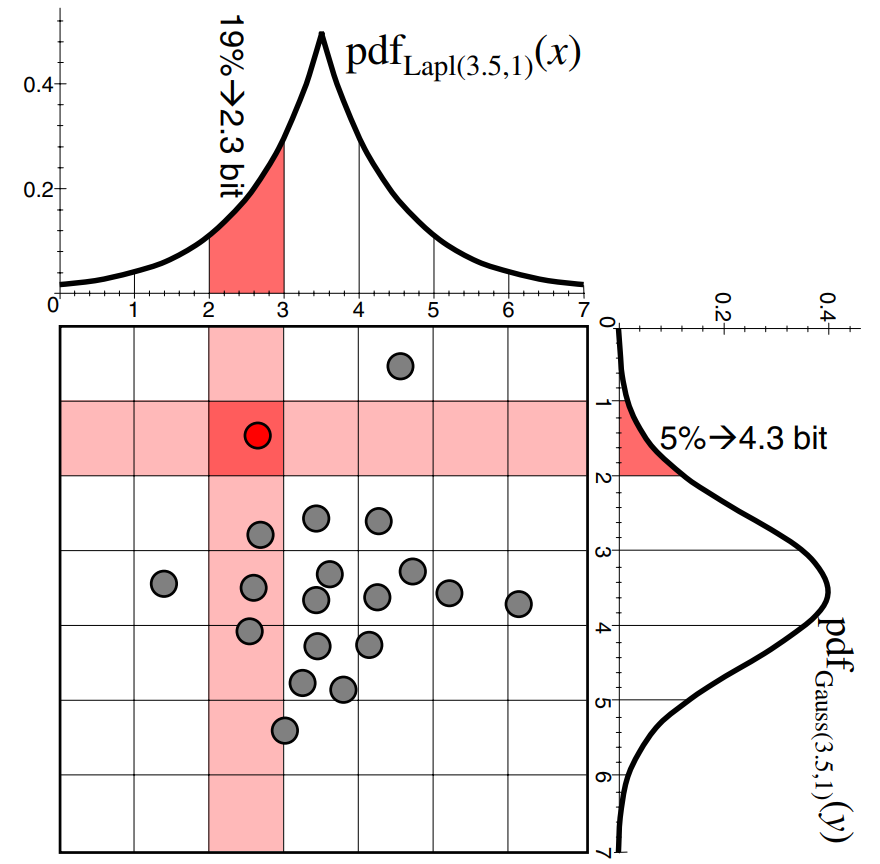
\includegraphics[width=\linewidth]{imgs/vac}
  \caption[]{Example of VAC\cite{Bohm2006-ts}}
  \label{fig:vac}
\end{figure}

\subsection{RF - Robust Fitting}
The Robust Fitting sub-algorithm deals with outliers in the input clusters. The fitting algorithm employs the VAC criterion to determine if a point is adequately described by the characteristic distribution of the cluster or if it makes more sense to not count that specific point as belonging to (any or this) specific cluster. An example of how a conventional clustering might work in finding a characteristic distribution as opposed to how the RF algorithm estimates its fitting using the VAC criterion can be found in figure \ref{fig:robust_estimation}. But the sole introduction of the VAC criterion to measure goodness does not yet incorporate outlier detection.

\begin{figure}
  \centering
  \noindent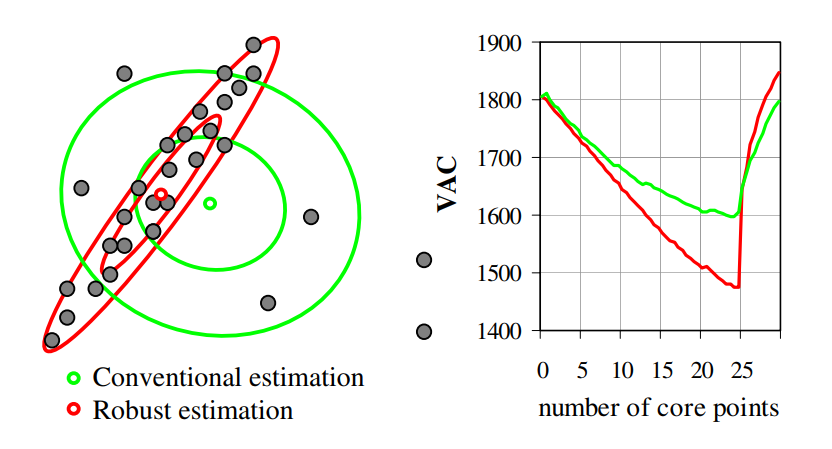
\includegraphics[width=\linewidth]{imgs/robust_estimation}
  \caption[]{Conventional and robust estimation\cite{Bohm2006-ts}}
  \label{fig:robust_estimation}
\end{figure}

Instead, RF derives its robustness regarding outliers from the fact that the conventional way to estimate the covariance matrix $ \Sigma $ is by computing a matrix $ \Sigma_C $ from the points $ \vec{x} \in C $ by averaging
\[ \Sigma_C = \frac{1}{|C|} \sum_{\vec{x} \in C} (\vec{x} - \vec{\mu}) \cdot (\vec{x} - \vec{\mu})^\text{T} \]
whereas RF doesn't solely use arithmetic means but also tries the coordinate-wise median (the median of $ (\vec{x} - \vec{\mu}_{R_i}) \cdot (\vec{x} - \vec{\mu}_{R_j}) $ over all $ \vec{x} $) yielding the robust covariation matrix $ \Sigma_R $.

Given the conventional covariance matrix $ \Sigma_C $, by Principle Components Analysis (PCA) one could obtain the orthonormal Eigenvector matrix $ V $, the decorrelation matrix, and the diagonal matrix $ \Lambda $, containing all Eigenvalues, with $ \Sigma_C = V \Lambda V^\text{T} $. Using the property of diagonal dominance (ie all diagonal elements are greater than the sum of the other values in their respective row), one could then measure the distance between any two points $ \vec{x} $ and $ \vec{y} $ by using the Mahalanobis distance\cite{Mahalanobis1936-wy} defined by $ V $ and $ \Lambda $:
\[ d_{\Sigma_C}(\vec{x}, \vec{y}) = (\vec{x} - \vec{y})^\text{T} \cdot V \cdot \Lambda^{-1} \cdot V^\text{T} \cdot (\vec{x} - \vec{y}) \]

The robust covariance matrix $ \Sigma_R $ does not necessarily have the diagonal dominance property. However, this can easily be fixed by adding a matrix $ \varPhi \cdot I $ to the covariance matrix. $ \varPhi $ should naturally be chosen as the maximum difference of all the column sums and their corresponding diagonal element. The authors also add a small amount on top of that (in their example 10\%), but it's not really clear why that added value would be needed, as even
\[ \varPhi_{naive} = \max_{0 \leq i < d} \left\{ \left( \sum_{0 \leq j < d, i\neq j} (\Sigma_C)_{i,j} \right) - (\Sigma_{C})_{i,i} \right\} \]
should be enough to satisfy the diagonal dominance property. They do however add that 10\%, which means the suggested value in the original paper is
\[  \varPhi = 1.1 \cdot \varPhi_{naive}. \]

The estimation of a robust covariance matrix does not mean that this matrix is actually used as the descriptive matrix of the cluster, however - the decision about which matrix to use is, as expected, made by calculating the VAC of both $ \Sigma_C $, $\Sigma_R $ and of several candidate matrices and finally choosing the one yielding the lowest VAC.

Once the covariance matrix with the lowest VAC is found, all points are first deemed outliers and then iteratively inserted into the set of cluster points (by order of their Mahalanobis distance from the distribution center), with accompanying VAC scoring at each step. Once a (local) minimum is reached, the process stops and the cluster and outliers are then returned to the next RIC sub-algorithm, CM.

\subsection{CM - Cluster Merging}
The Cluster Merging algorithm is likely the computationally costliest part of the RIC process as it compares each cluster with every other cluster for possible merging using the VAC criterion again, or simply checking if
\[ VAC(C_i \cup C_j) < VAC(C_i) + VAC(C_j) \]
for all $ C_i,C_j \in \mathcal{C},i \neq j $. Getting the VAC score of a merged cluster seems only possible by building a new set of points from the previous two clusters and running the whole RF algorithm on that set again.

The CM part of the algorithm also comes with the option of going further down the search tree to get out of a local minimum. It will then merge clusters even if
\[ VAC(C_i \cup C_j) \geq VAC(C_i) + VAC(C_j) \]
for a given $ t $ iterations. If it actually does find to have been in a local minimum, the counter will naturally reset to 0.

\section{Experiments}
\label{sec:exp}
RIC is tested on two different sets of synthetic data and on two different sets of real data. RIC found all the correlational, Laplacian and Gaussian clusters in the synthetic data sets, the input being provided by either K-means or DBSCAN\cite{Ester1996-rh}. RIC manages to correctly identify more than 98\% of the noise objects in the data sets and reduces the initial VAC score by about a quarter each. The provided runtimes for both data sets are provided and discussed below in section \ref{sub:run}.

Further evaluation is provided by running RIC on a 14-dimensional real world metabolic data set. Clustering in this biomedical instance can provide help in diagnosing disorders, if the algorithm can cluster both the healthy control group and the test group with disease correctly. For that reason, in this situation as further points of comparison \textit{impurities} in the clusters are counted - impurities being wrongly assigned groups for the known distribution, ie the sum of statistical type I and type II errors. As expected, RIC is able to beat both spectral as well as K-means clustering by achieving a lower VAC, even with both other clustering algorithms being provided with the correct number of clusters to identify. More importantly, however, is RIC's far superior number of impurities (mostly ill datapoints ascribed to the healthy cluster), usually making only about a third of the errors that K-means and spectral achieve alone.

The fourth example provided concerns retinal images of cats in various states of health. The images are encoded as a 7-dimensional data set with more than 21 thousand instances, which RIC (again using K-means as a starting point) clusters into 13 clusters, all of which are correlational, and two of which describe actual, studied, biological meaningful relationships, namely the "Müller cells" and "rod photoreceptors". As RIC's pretense was to provide meaningful clusters without user-input, and, as such, without relying on the user's specific domain knowledge, this can be taken as a sign that it at least partially reached its goal.

\section{General Criticism}
\label{sec:crit}
As the lead author himself confirms in later works\cite{Bohm2008-eh}\cite{Bohm2010-uu}, the clustering output of RIC strongly depends on the quality of the initial clustering and the cluster model is limited to linear attribute correlations. They're also limited to the list of predefined PDFs, though that might not be too much of a limitation, as, in theory, new PDFs are supposed to be added quite easily. Further, there's a reason that there's only a limited to supply of deeply researched and named density functions to begin with, namely that they're readily applicable to a big enough subset of problems. Natural processes that need much more elaborate models also are clearly not in scope of the RIC framework.

\subsection{Runtime Analysis}
\label{sub:run}
The paper does not contain an explicit runtime analysis of RIC in general or its sub-algorithms. It is, however, relatively easy to see that the VAC calculation itself should take at most linear time as it's only adding up the total size of an encoded input. The Robust Fitting part can probably be assumed to also need only linear time, whereas the Cluster Merging algorithm almost certainly grows quadratically at least in the worst case.

The experimental runtimes that can be taken from the paper (147s for 4751 objects in 2 dimensions and 567s for 7500 objects in 3 dimensions) also seem suggestive of a quadratic growth rate, as an input of $ 7500 \cdot 3 = 22500 $ integers, about 2.4 times as many as $ 4751 \cdot 2 = 9502 $ integers takes roughly 3.9 times the time to process.

\begin{table*}
  \caption{Comparison of RIC with other information-theoretic clustering algorithms}
  \label{tab:comp}
  \begin{tabularx}{\textwidth}{rlllXXl}
  	\toprule
  	                    & parameter-free & runtime analysis              & input data          & clustering strategy & clusters detected                                       & year \\ \midrule
  	                RIC & yes            & $ O(n^2)^{\beta} $            & matrix              & input-refining      & Gaussian, Laplacian, Correlational, others$ ^{\alpha} $ & 2006 \\
  	              PaCCo & yes            & $ O(n) < x < O(n^3)^{\beta} $ & graph (weighted)    & bisecting             & Gaussian, others$ ^{\alpha} $                           & 2011 \\
  	minCEntropy($ ^+ $) & no             & $ O(n^2) $                    & matrix              & proprietary         & Gaussian                                                & 2010 \\
  	              ROCAT & yes            & $ O(n) $                      & matrix              & bisecting         & not applicable                                          & 2014 \\
  	               PICS & yes            & $ O(n) $                      & graph (attributed)  & bisecting         & not applicable                                          & 2012 \\
  	            INCONCO & yes            &           $ O(n)^\beta $                    & matrix (attributed) & bisecting                    & Gaussian                                                & 2011 \\
  	                NIC & yes            &     $ O(n^2) $                          &    matrix                 &      greedy sequential k-means               &      non-convex                                                   & 2010 \\
  	                VoG &  yes              &     $ O(n)^\gamma $                          &     graph                &      multiple               &          not applicable                                               & 2014 \\ \bottomrule
  	\multicolumn{7}{l}{$ ^{\alpha} $ user-defined PDFs are explicitly mentioned as desired extensions to the algorithm}                                                               \\
  	\multicolumn{7}{l}{$ ^{\beta} $ estimate, as the respective authors did not provide an explicit runtime analysis} \\
    \multicolumn{7}{l}{$ ^{\gamma} $ the average case with $ n $ being the numbers of edges on the graph}
  \end{tabularx}
\end{table*}

\subsection{Edgecases}
It would have been interesting to see how the RIC framework reacts to random or exactly equally distributed input. Would it see structure in the noise regardless? Would the CM method make initial bad K-means clustering on such data more deterministic? Sadly, there are no examples included in the paper that can act as a kind of control group.

\section{Comparison with other Algorithms}
\label{sec:comp}
In this section, we'll compare how RIC fares against some of the other clustering algorithms introduced in the seminar, eg PaCCo\cite{Mueller2011-hd}, minCEntropy\cite{Vinh2010-tc}, ROCAT\cite{He2014-uf}, PICS\cite{Akoglu2012-vz}, INCONCO\cite{Plant2011-wy}, NIC\cite{Faivishevsky2010-uk}, VoG\cite{Koutra2014-up} and Subdue\cite{Ketkar2005-zs}. The categorical results of these comparisons are provided succinctly in table \ref{tab:comp}.

\subsection{PaCCo}
PaCCo is a weighted graph-based algorithm employing the information-theoretic MDL principle to check the goodness of a clustering just like RIC does, including the Huffman coding structure along a cluster PDF. Different from RIC, however, PaCCo in general assumes Gaussian clusters, but other PDFs can be added by the user. A further similarity is the fact that both algorithms work without user-input. PaCCo however comes with its own bisecting K-means strategy, so its input really are completely unordered and unclustered data.

PaCCo's runtime efficiency is not explicitly stated, other than being "super-linear". In tests against Zelnik-Manor and Perona's parameter-free SpectralZM algorithm\cite{Zelnik-Manor2004-rx}, which has a runtime of $ O(n^3) $, PaCCo outpaced SpectralZM with ease. Its real runtime efficiency will thus lie somewhere in-between.

In conclusion, with PaCCo introduced significantly later than RIC, and having a different input assumption, the RIC framework still holds up surprisingly well in comparison.

\subsection{minCEntropy$ (^+) $}
The focus of minCEntropy lies not on producing a single clustering solution to a given data set, but instead realizes that data can often be interpreted in more than one way (eg data that can be used for facial recognition/authentication could also be used to identify looking direction). The algorithm's goodness criterion seems different from all the other criteria employed throughout this paper - instead of referencing the MDL principle the authors choose to minimize the conditional entropy left in the data, or in other words, maximize the average intra-cluster similarity (hence the name). Of course, concentrating on maximizing intra-cluster similarity will invariably make it easier to succinctly describe a given cluster - in other words, minimizing the description length needed.

The included complexity analysis puts emphasis on the fact that although initializing the required kernel matrix takes up to $ O(n^2) $ time, further updating to reach an optimal clustering takes only linear time and converges quickly.

Then, minCEntropy$ ^+ $ is the extension of minCEntropy to find the above mentioned alternative clusterings when given a clustering to explicitly exclude. There's also a further extension minCEntropy$ ^{++} $ that can exclude multiple clusters.

No iteration of the algorithm works completely parameter-free.

\subsection{ROCAT}
ROCAT is a pretty young, parameter-free approach to clustering, using the MDL principle (though expressed as a question of entropy like with minCEntropy above), and focusing on subspace clusters for categorical (ie not numerical) data. As ROCAT deals with categorical data, a defining cluster probability distribution like a Gaussian curve is not really applicable. Clusters built by ROCAT over a matrix view of the attributive data are always shaped rectangular.

ROCAT's runtime efficiency grows linearly with $ n $, quadratically with dimensionality, so it's one of the most efficient algorithms discussed until now.

\subsection{PICS}
PICS is a parameter-free graph-clustering algorithm that does not solely cluster on connectivity information but also takes node attributes into account. Naturally, PICS also relies on an MDL criterion to decide if a split of the biggest identified cluster brings a better description of the data (similar to the approach used by PaCCo above).

\subsection{INCONCO}
INCONCO is a parameter-free clustering algorithm with much the same premise as PICS, only that it is not based on graph data with attributes, but instead on vector data with mixed-type attributes.

Where RIC uses the Robust Fitting method instead of PCA to make its clustering less sensitive to outliers, INCONCO extends Cholesky decomposition\cite{Golub1996-ak} as it's more efficient than PCA and yields better results. The usage of an MDL criterion for decisions regarding goodness of fit at each step of the bisecting algorithm going through the input data set does not come as a surprise anymore.

There is no explicit theoretical runtime analysis given, but from the runtimes reported, INCONCO seems extremely efficient when looking at the number of points processed, with much of it probably due to a large but constant overhead.

\subsection{NIC}
NIC is a parameter-free framework that can find clusters independently of their underlying structure utilizing the MeanNN differential entropy estimator. NIC is certainly different in that it can even find clusters consisting of points non-convex sets (eg concentric circles), a feat that RIC would not be able to accomplish without being fed a complex user defined distribution first.

\subsection{VoG}
The premise of VoG is the description of large graphs using a certain vocabulary (eg stars, chains, bi-partite cores). So not only shall clusters in the graph be recognized, but also be described by their most descriptive characteristic. By then examining the frequencies with which the predefined structures in the vocabulary appear in the graph and the most notable structures altogether, one can make some meaningful abstractions of the underlying real world structure (eg finding the two groups comprising a Wikipedia edit war). 


\section{Conclusion}
\label{sec:conc}
In the end, especially against competitors that were introduced significantly later and which could build upon a larger body of work with much the same direction, the RIC framework still fares surprisingly well. It is one of the few algorithms that comes pre-equipped with more than just the regular Gaussian PDF (of course, Gaussian distributions still play one of the most significant roles in data description across all fields). Its runtime complexity is not the most amazing thing about the framework, but still holds up against much of the competition. As we've seen under section \ref{sec:crit}, there are some valid criticisms to be aware of, but as the real world examples have shown, any clustering algorithm that can identify known relations consistently and, as such, can be used to find new relationships in data is a step in the right direction.

Adding into that the fact that the RIC framework provides exactly that, a framework that can profit from the fact that clustering elsewhere might get better and as such provide better input to be enhanced by the information-theoretic principles that guides it, the findings by Böhm et al. certainly advanced the area of research they set out to advance.

\section*{Acknowledgments}
The author would like to thank Dr. Bianca Wackersreuther for providing input and help whenever needed and conducting the seminar in a well-received and professional manner. Next, Prof. Christian Böhm, both for co-authoring the discussed paper in the first place, and then giving me the opportunity to engage with the topic for this course. Lastly, the other participants in this seminar, for providing constructive criticism after my talk without which this discussion paper wouldn't have been possible.

\bibliography{sources.bib}{}
\bibliographystyle{plain}

\end{document}
